\documentclass[%
xelatex,
	oneside,		% Single side print
	12pt,			% Font size
	parskip=half,	% Half line skip between paragraphs
	headsepline,	% Line after header
	footsepline,	% Line before footer
	abstracton,
	chapterprefix=true% like in standard class "report"
    appendixprefix=true]
{scrreprt}
\usepackage[english]{babel}

\usepackage{rwufont}
\usepackage[pdfusetitle]{hyperref}
\title{Master Thesis}
\author{Viplav Setia}
\usepackage{graphicx}
\usepackage{nomencl}
\makenomenclature
\renewcommand{\nomname}{List of abbreviations, formulas and indexes}
\usepackage{blindtext}
\begin{document}
	

	
\section*{\Large\normalfont\bfseries Declaration}
	\addcontentsline{toc}{chapter}{Declaration}

I, Viplav Setia, born on 04.04.1995 in New Delhi, India, assure that I have done this work independently.All sources and references used for the completion of this
thesis have been listed and cited accordingly. This thesis work was done in
partial fulfillment of the requirements for the award of the degree of Master of
Science in Mechatronics at Hochschule Ravensburg Weingarten and has not been
used or submitted elsewhere for award of a degree, grade or in any publication. \newline


\rule{5cm}{.4pt}

Viplav Setia \newline
Friedrichshafen, 31 January 2020
\clearpage

		\section*{\Large\normalfont\bfseries Acknowledgement}
		\addcontentsline{toc}{chapter}{Acknowledgement}

I would like to express my heartfelt
gratitude to Prof Dr.-Ing Benedikt Reick and Prof Dr. rer. nat. Markus Pfeil for guiding me through the completion of my Master thesis and for their valuable
suggestions.

I am extremely thankful to ALTEN GmbH and their colleagues who gave me this opportunity and the resources to do this thesis at their office branch in Friedrichshafen. They also supported me with their knowledge,  expertise and created a pleasant working environment, without which it would have been difficult to move forward with this project.

Also, many thanks to my family and friends for their constant encouragement.				
	\clearpage
		\section*{\Large\normalfont\bfseries Abstract}
		\addcontentsline{toc}{chapter}{Abstract}

The automotive industry is changing rapidly to new technologies like electromobility and autonomous driving. All major companies like Daimler, BMW, Tesla, Bosch, etc. are investing heavily to bring electric cars to the market and develop prototypes for autonomous driving. To support this change, middleware is required which is used as a means of data exchange between various sensors, control systems and actuators. The focus of this thesis is to test the new versions of the middleware Robot Operating System(ROS\nomenclature{ROS}{Robot Operating System}) which offer support for embedded and real time systems. To test the version micro-ROS, a demonstrator was built using a STM32 microcontroller with a Nuttx Real-Time Operating System(RTOS\nomenclature{RTOS}{Real-Time Operating System}) installed to show the data transfer of a pressure sensor. To test the real-time performance for this version, an algorithm was created to test the delay in data transfer with different data sizes. To test the real-time performance of ROS2, an inverted pendulum demo was used and its simulation was visualised on a Linux system enabled with real-time capabilities. Finally, a model using the Gazebo robot simulator was developed to explore ADAS applications using a camera and a LIDAR sensor as an example to show the data transfer using ROS2 for the automotive industry.
\clearpage

	\addcontentsline{toc}{chapter}{List of abbreviations, formulas and indexes}
	
	

\printnomenclature
	

	\tableofcontents
	\chapter{Introduction}
  Dummy Text 
\begin{figure}[ht]
\begin{center}
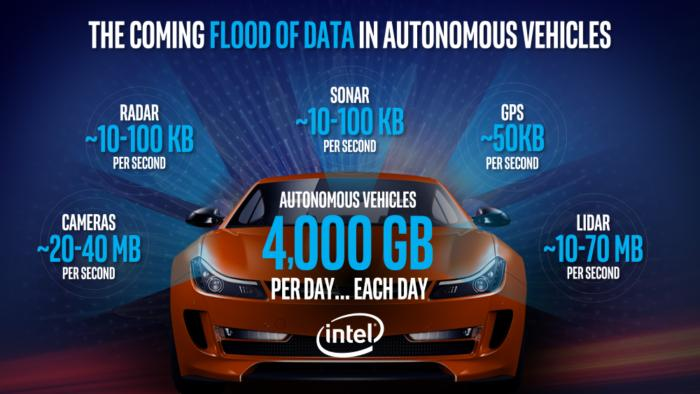
\includegraphics[scale=.5]{fig/autonomous-vehicle-data-intel-100697604-large.jpg}
\caption[Data Stats in Autonomous Cars]{Data Stats in Autonomous Cars\cite{dumm}}
\label{fig:dumm}
\end{center}
\end{figure}  
  
     \section{Motivation}	
			Why?
	 \section{Objectives}
	 Tasks
	 \section{Robot Operating System(ROS)}
	 ROS
	 History
	 ROS2
	 micro-ROS
	 
	 
	\chapter{Literature Research}	
	
	\section{ROS2 Concepts}
	Node
	Topic
	Message
	DDS
	OS
	Discovery

	\section{ROS1 vs ROS2}	
	
	\section{Embedded Systems}
	STM32 Micro-controller
	Features
	Communications : 
	IP
	Serial
	
	\section{Real Time Systems}
		Requirement
		Types : Soft
		Firm
		Hard
		
	\section{Previous Research Results}
	
		
	
	
	
	\chapter{Test Setup}
	
	\section{Testing micro-ROS}

	\subsection{Components}
	\subsection{Procedure}	

	\section{Testing ROS2}
	\subsection{Components}
	\subsection{Procedure}	


		\chapter{Results}
		\section{Latency Analysis in micro-ROS}
		\section{Latency Analysis in ROS2}
		
		\chapter{ADAS Applications using ROS2}
		\section{Lane Detection using Camera}
		\section{Auto Stop using LIDAR}
		\section{Driver Control using Keyboard}
		
		
		\chapter{Conclusion and Future Scope}
		\addcontentsline{toc}{chapter}{List of Figures}
	\listoffigures
	\addcontentsline{toc}{chapter}{List of Tables}
	\listoftables
		
		\addcontentsline{toc}{chapter}{Bibliography}
\bibliographystyle{plain}		
\bibliography{thesis}





\end{document}
